\documentclass{article}
\usepackage{graphicx}
\usepackage[margin=1in]{geometry}
\usepackage{indentfirst}
\usepackage{enumerate}

\begin{document}
\title{Project Testing and Delivery Document}
\author{Team D}
\date{\today}

\maketitle

\vspace*{3.5in}
\begin{table}[htbp]
\caption{Team}
\begin{center}
\begin{tabular}{|r | c|}
\hline
Name & ID Number \\
\hline\hline
Stefanie Lavoie & 1951750 \\
Pinsonn Laverdure & 9684352 \\
Ghislain Ledoux & 6376320 \\
Rigil Malubay & 6262732 \\
Philippe Milot & 9164111 \\
Christopher Mukherjee & 6291929 \\
\hline
\end{tabular}
\end{center}
\end{table}

\pagenumbering{gobble}% Remove page numbers (and reset to 1)
\clearpage

\begin{table}[htbp]
\caption{Revision History}
\begin{center}
\begin{tabular}{|c | c | c | c| }
\hline
Date & Version & Description & Author \\
\hline\hline
30/07/13 & 0.1 & Set up initial layout of deliverable & Philippe Milot \\
\hline
30/07/13 & 0.2 & Finished Section 2.2.1 & Philippe Milot \\
\hline
30/07/13 & 0.28 & Added initial cost estimate to Section 4 & Christopher Mukherjee \\
\hline
30/07/13 & 0.38 & Finished Section 1 & Christopher Mukherjee \\
\hline
04/08/13 & 0.39 & Started Section 3.2 & Stefanie Lavoie \\
\hline
06/08/13 & 0.41 & Added Gantt Chart to Section 4 & Christopher Mukherjee \\
\hline
11/08/13 & 0.43 & Finished Sections 2.1 \& 2.2.3 & Philippe Milot \\
\hline
11/08/13 & 0.43 & Added feature of map panel to Section 3.1 & Rigil Malubay \\
\hline
12/08/13 & 0.44 & Completed Section 3 & Stefanie Lavoie \\
\hline
12/08/13 & 0.45 & Finalized Cost Estimate in Section 4 & Pinsonn Laverdure \\
\hline
13/08/13 & 0.46 & Finished Section 4 & Christopher Mukherjee \\
\hline
13/08/13 & 0.48 & Reviewed \& edited entire document & Christopher Mukherjee \\
\hline
\end{tabular}
\end{center}
\end{table}

\clearpage

\tableofcontents
\clearpage

\pagenumbering{arabic}% Arabic page numbers (and reset to 1)

\section{Introduction} % COMPLETE

% [The introduction of the document provides an overview of the entire document, briefly introducing what are its goals, and what information is to be found in it.]

This document will describe in detail the testing process and final delivery for the Vessel Monitoring System which was developed in the context of the COMP354 course. This document includes a report on which items were tested and which were not, descriptions of the unit testing and requirements testing that was performed, a description of stress testing that could have been performed (but was \emph{NOT} performed), an installation manual and users manual, and a final cost estimation for the entire project.

\break

\section{Testing Report}

% [This section presents all the testing activities undertaken on the final product, as well as all the individual test cases used.]

\subsection{Test Coverage}

\subsubsection{Tested Items} % STATUS: COMPLETE

% [List all tested items, along with the test cases that were applied on this item. For each test item, explain why it was necessary to test it. For instance, all features listed as requirements for each build is a mandatory test item. In addition, identify at least five units (i.e. classes/methods) and explain why they require unit testing due to their importance in the implementation through their frequency of use and/or the severity of the impact of their misbehavior. You can categorize your tested items, e.g. “Requirements”, “Units”, etc.]

\paragraph{VSF file parsing.} Test that valid VSF files were correctly parsed. Test that invalid VSF files cause a helpful program error to be printed.

\paragraph{Client-side connection.} Test that the simulator returns a helpful error message when attempting to connect to a non-existing VMS. Test that the simulator correctly connects to an existing VMS.

\paragraph{Time management on simulator side.} Test that the simulator properly respects the \verb|TIMESTEP|, \verb|STARTTIME|, and \verb|TIME| instructions in the VSF file.

\paragraph{Server-side connection.} Test that the VMS can bind to a proper host and port number. Test that the VMS returns a helpful error message when trying to bind to an already-bound host and port number.

\paragraph{Client data validation.} Test that any invalid data coming from a connected client will be silently ignored by the VMS.

\paragraph{VMS Update Rate.} Test that the VMS display is updated as soon as new information comes in. Test that the VMS display is updated at a fixed, regular rate when no data is coming in.

\paragraph{Out-of-range Vessels.} Test that the VMS ignores any vessel located outside its tracking range. Test that the VMS removes any vessel from its list of tracked vessels as soon as it moves out of range.

\paragraph{VMS Table Display.} Test that the VMS displays all possible information about tracked vessels, namely: ID, type, X-Y coordinates, speed, course, distance from center of radar, last updated time, and risk level.

\paragraph{VMS Table Filtering.} Test that the VMS properly hides rows of vessels with a type unselected in the filter list.

\paragraph{VMS Table Sorting.} Test that all rows are ordered by the currently-selected column in the table.

\paragraph{Map View Display.} Test that the VMS can display the latest received information in a 2D map containing all vessels as arrows.

\paragraph{Map View Filtering.} Test that the VMS properly hides vessels with a type unselected in the filter list.

\paragraph{VMS Access Levels.} Test that the following features are only available when logged-in as administrator: Filtering, Sorting.

\paragraph{Alert Highlighting.} Test that all vessels involved in a low-risk alert are highlighted in yellow in the table view, and display a yellow circle around the vessel at the low-risk range in the map view. Test that all vessels involved in a high-risk alert are highlighted in red in the table view, and display a red circle around the vessel at the high-risk range in the map view.

\paragraph{Alert Icon Indicator.} Check that the upper-left circle always indicates the most serious alert level at any given time.

\subsubsection{Untested Items of Interest} % STATUS: COMPLETE

% [List all untested items that you find would necessitate testing. Explain how it could be tested, and why it would be important to test.]

\paragraph{Command-line argument parsing}. We did not write extensive tests for command-line argument parsing, even though it can be considered input to the system (and therefore unsafe). It would be important to test this more thoroughly in the future.

\paragraph{Large client update data}. We did not test the case when client data exceeds 1mb in size (example: an extremely large number of update data sent sequentially in one shot). Theoretically, it would cause the data to be truncated at 1mb, and therefore result in some of the updates to be flagged as ``invalid'' and ignored.

\subsection{Test Cases}

% [Description of all the test cases applied on the tested items using various techniques and testing different aspects of the system. The following sections are mandatory testing perspectives. Other sections can be added to provide appropriate additional testing perspectives. All test cases must be presented as to be reproducible, with the exact data and procedure to convey the test, as well as the expected result.]

\subsubsection{Unit Testing} % Status: COMPLETE

% In your system, identify 2 testable units (classes, modules or subsystems)

% [For each of these two units, include a list of test cases. Explain what techniques were used to derive these tests, e.g. black box/equivalence partitioning, white box/basis path, etc.]

\paragraph{VesselTest}

The \verb|Vessel| class was extensively tested using JUnit. All test cases were designed under the black box principle. The test cases were:

\subparagraph{JavaBean functionality}
Test all basic accessor/mutator methods.

\subparagraph{Coordinate calculation}
Project current coordinates based on last-known coordinates, course, and time elapsed.

\subparagraph{Error conditions}
Test that the class properly throws exceptions whenever bad data is supplied.

\paragraph{RadarMonitorTest}

The \verb|RadarMonitor| class was extensively tested using JUnit. All test cases were designed under the black box principle. The test cases were:

\subparagraph{Manual refresh}
Check that when the RadarMonitor is manually refreshed, all its observers are also refreshed.

\subparagraph{Manual update}
Check that when the RadarMonitor is manually fed new data, the data is forwarded to all observers.

\subparagraph{Active alert detection}
Check that when the RadarMonitor is manually fed new data, any alerts triggered by the update are properly detected and observers are notified.

\subparagraph{Passive alert detection}
Check that when vessels passively drift toward each other over time, all relevant alerts are detected and observers are notified.

\subparagraph{Radar range}
Check that when ships drift outside the radar range, they are no longer tracked by the monitor.

\subsubsection{Requirements Testing}

% [For each tested requirement, include a list of test cases presented in the form of a concrete scenario of system usage and expected system reaction.]

\paragraph{Requirement 1: Vessel list displays latest information.}


\subsubsection{Stress Testing} % STATUS: COMPLETE

% Describe potential extreme situations of system usage. Describe the design of tests that would verify system performance under these extreme conditions. Do not perform the tests.

The system was stress-tested with up to 150 vessels tracked simultaneously, using three distinct connected clients. The system has not been proven to be reliable beyond these limits.

\section{System Delivery}

% [This section provides instructions as to how to install and use the software.]

\subsection{Installation Manual}

This manual will explain the procedures that need to be done in order to allow the Vessel Monitoring System run on the user's computer. Since Java is a cross-platform language, this program will run on any platform (Windows, Mac, or Linux).

\paragraph{Install Java \\}
\begin{enumerate}[(a)]
  \item By going on the Java website ( http://www.java.com/en/download/ ), you will be able to download the lastet version of Java. It is important that you download Java Version 7 or higher in order for the program to run.
	\begin{figure}[!htb]
	\centering
	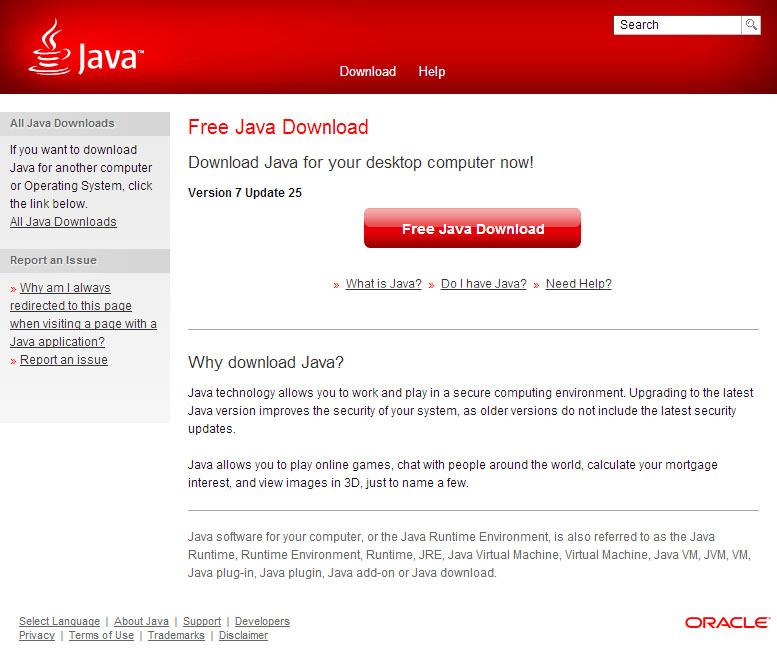
\includegraphics[scale=0.55]{images/javaInstall1.jpg}
	\end{figure}
\pagebreak
  \item Once the download is complete, run the executable file to install Java and follow the on-screen instructions.\footnote{Screenshots are provided for the Windows version of the Java installer.}
	\begin{figure}[!htb]
	\centering
	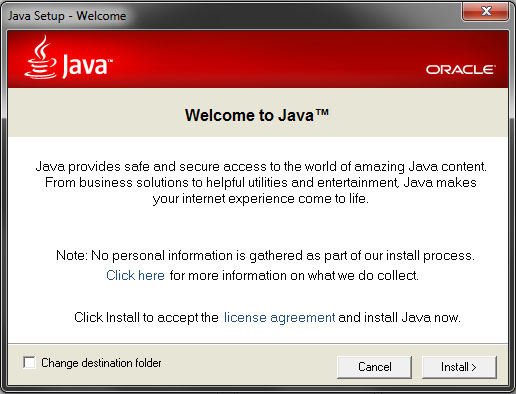
\includegraphics[scale=0.6]{images/javaInstall2.jpg}
	\end{figure}
  \item Once the installation is complete, you will get pop up message stating that Java has been successfully installed on your computer.
	\begin{figure}[!htb]
	\centering
	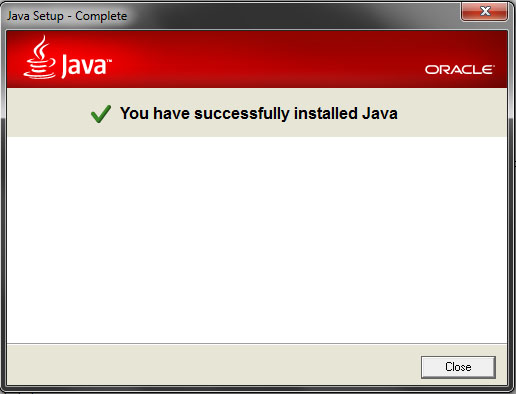
\includegraphics[scale=0.6]{images/javaInstall3.jpg}
	\end{figure}
\end{enumerate}

This is the only installation required in order to run the Vessel Monitoring System correctly.
\clearpage

\subsection{Users Manual}
\paragraph{Brief Overview \\ \\}

The Vessel Monitoring System(VMS) is a Java-based application that allows its users to check the positions of various types of vessels. This application can only be accessed by current valid users and administrators of the program. To run the program, you will need the two different jar files for the Vessel Monitoring System and the Radar Simulator. The Vessel Monitoring System should be run first, followed by the Radar Simulator once the user has logged into the VMS.

\subsubsection{Vessel Monitoring System}
\paragraph{Login Screen \\ \\}
The Login screen is directly accessed as soon as the VMS program start. A valid password is required to be allowed to use the program. Only two access levels are available, normal user and administrator, both of which have separate passwords.% [Not sure if we should just say what the passwords are here??]

	\begin{figure}[!htb]
	\centering
	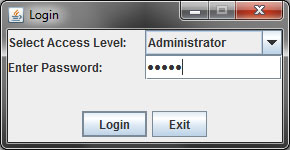
\includegraphics[scale=0.80]{images/userManual1.jpg}
	\end{figure}

\paragraph{Main Screen \\ \\}
After logging in, the Main Screen will appear. This is where all the important information will be displayed. The Main Screen will be different depending on the current user's access level. An administrator will have more options than a normal user. The main screen consists of:

\subparagraph{1) Menu bar \\ \\}

The menu is where the user can select to logout or exit the program.
	\begin{figure}[!htb]
	\centering
	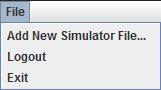
\includegraphics[scale=1]{images/userManual4.jpg}
	\end{figure}

If the logout option is selected, then the program will return to the Login Screen.\\

\pagebreak

\subparagraph{2) Table View Tab \\ \\}
In this view, the user can see a list of all the vessels detected by the radar. The color of each row depends on the type of alert this specific vessel is currently involved in. If the user has logged in as an administrator, the vessels can be ordered by any column in ascending or descending order by clicking the header cell at the top of each column in the table.

	\begin{figure}[!htb]
	\caption{Administrator Table View}
	\centering
	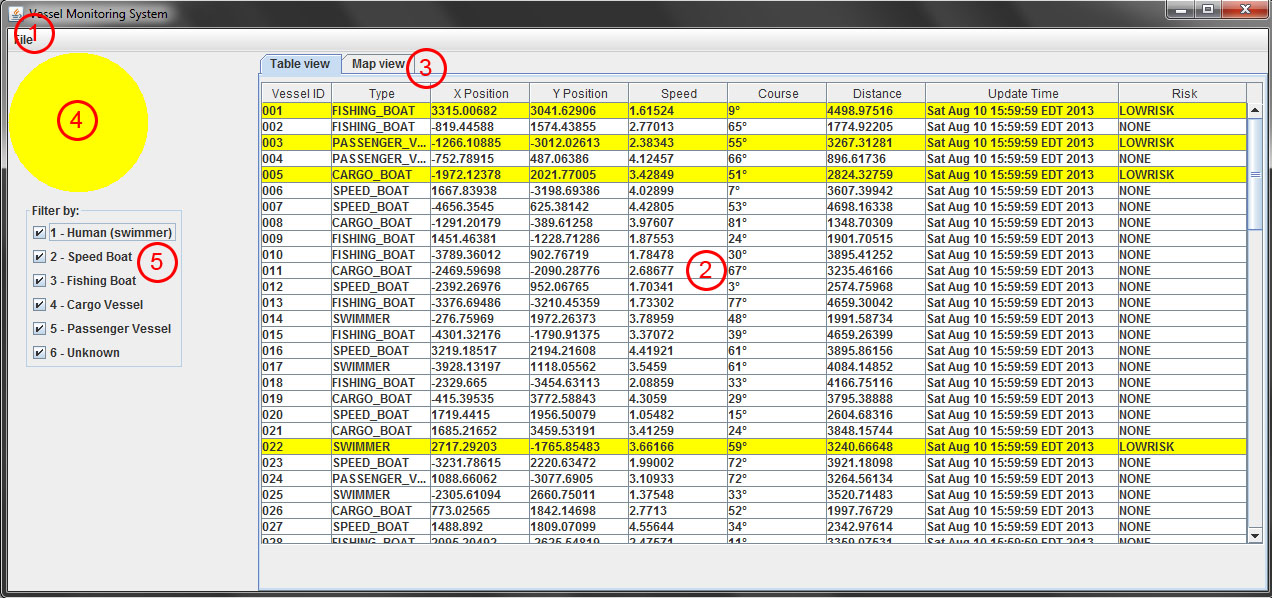
\includegraphics[scale=0.4]{images/userManual2_admin.jpg}
	\end{figure}

	\begin{figure}[!htb]
	\caption{Normal User Table View}
	\centering
	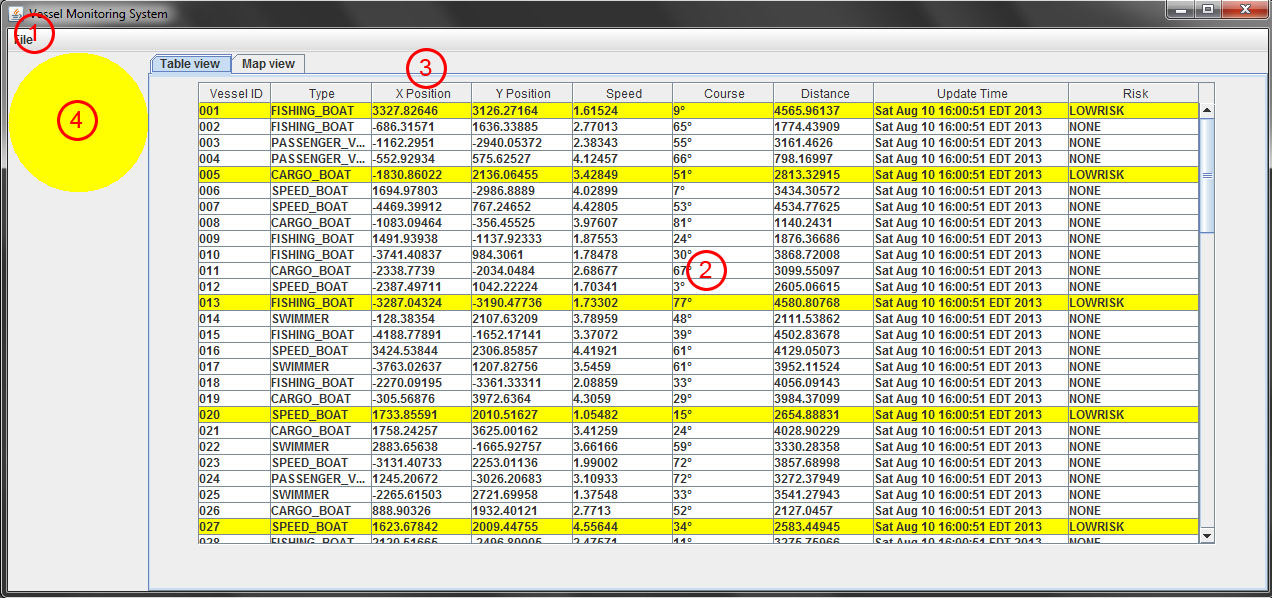
\includegraphics[scale=0.4]{images/userManual2_user.jpg}
	\end{figure}

\break
\subparagraph{3) Map View Tab \\ \\}
In this view, the user can see the vessels displayed on the map. Different type of vessels have different colors. The position of every vessel will be updated over time. The color and visibility of the circles around the vessels will change depending on the alert type of a vessel.
	
	\begin{figure}[!htb]
	\caption{Administrator Map View}
	\centering
	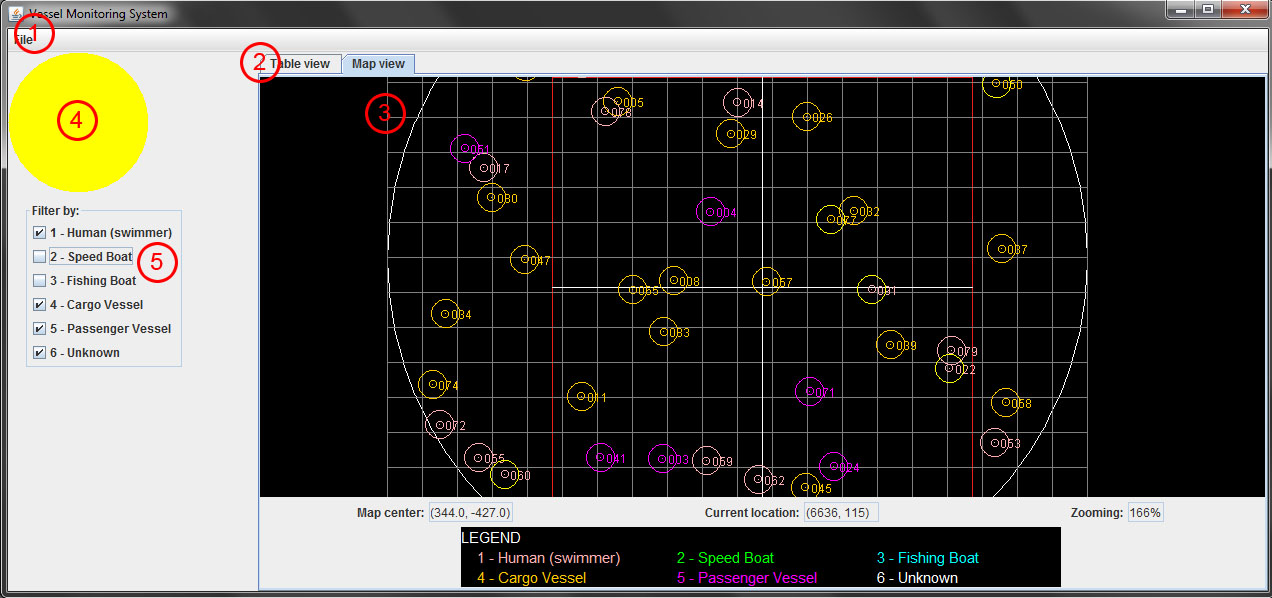
\includegraphics[scale=0.36]{images/userManual3_admin.jpg}
	\end{figure}

	\begin{figure}[!htb]
	\caption{Normal User Map View}
	\centering
	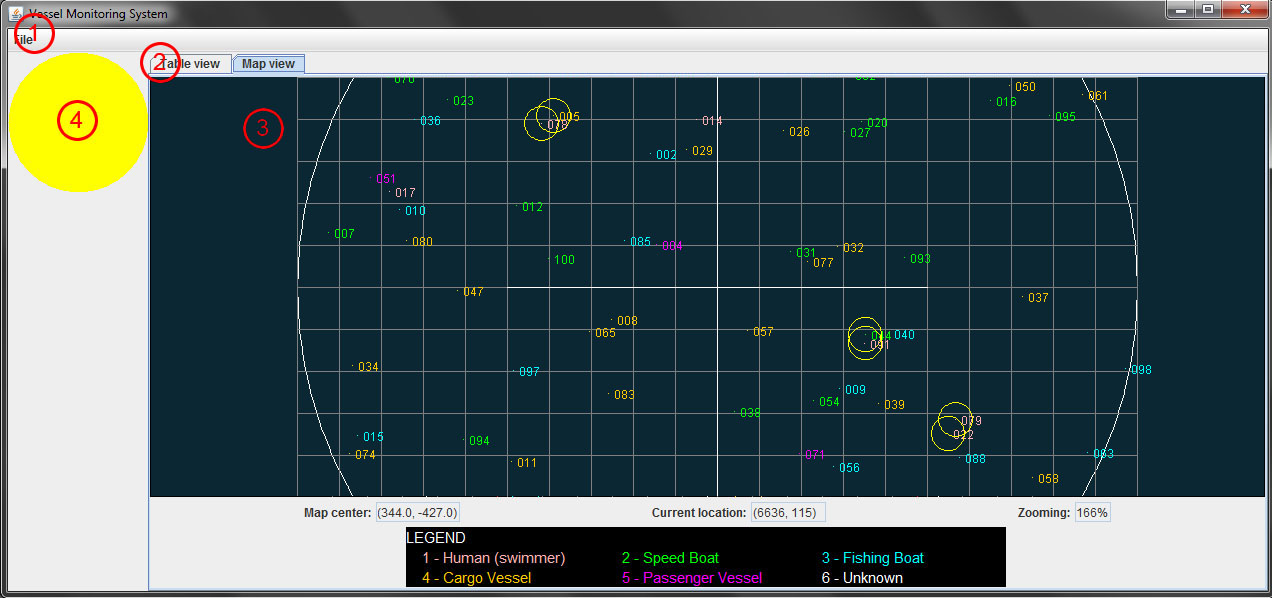
\includegraphics[scale=0.36]{images/userManual3_user.jpg}
	\end{figure}

There is also a zoom functionality in the map tab. It is enabled by scrolling the mouse forward (to zoom in) or backward (to zoom out) on the map area. Zooming is performed on the point of origin. There are two ways to change the point of origin. A user can either click on the map to quickly move the point of origin to the location of the click, or click and drag the map to the desired location. The map will only go within 5000 meters of the default point of origin.

\pagebreak
\subparagraph{4) Alert Indicator \\ \\}
The alert indicator always displays the color of the current most serious alert. A green circle indicates that all the vessels are a safe distance from one another. A yellow circle indicates that some vessels are very close to one another. A red circle indicates that some vessels are dangerously close to one another and that a collision may occur.\\

\subparagraph{5) Filters \\ \\}
This section is only available if the user has logged in as an administrator. The filters allow the user to hide/show certain types of vessels by deselecting/selecting the proper checkboxes.\\

\subsubsection{Radar Simulator}
The Radar Simulator must be run from the command-line after the user has logged into the Vessel Monitoring System. Using the command prompt, the user should navigate to the folder containing the jar files to run the application. Once in the correct folder, the following line must be written in order to run the Radar Simulator.

\begin{verbatim}
java -jar radarsimulator.jar --host localhost --port 11233 --input COMP354_50_demo_500.vsf
\end{verbatim}

Here, the host and the port are specific to the machine that is running the Radar Simulator. If both are running on the same machine, then the host should be "localhost" and the port number "11233". The vsf file listed above is an example of a vsf file located in the same folder as the jar files. The user can type the path of any vsf file followed by its complete name to run files in other directories.

\break

\section{Final cost estimate} % Status: Work in Progress

% [This shall consist of a table listing all components of all phases of this project, including the person hours cost of each component of each phase. This should include documentation, design, implementation and testing. Include the meeting minutes with action item and the time log as well]

\begin{figure}[!htb]
\caption{Gantt Chart}
\centering
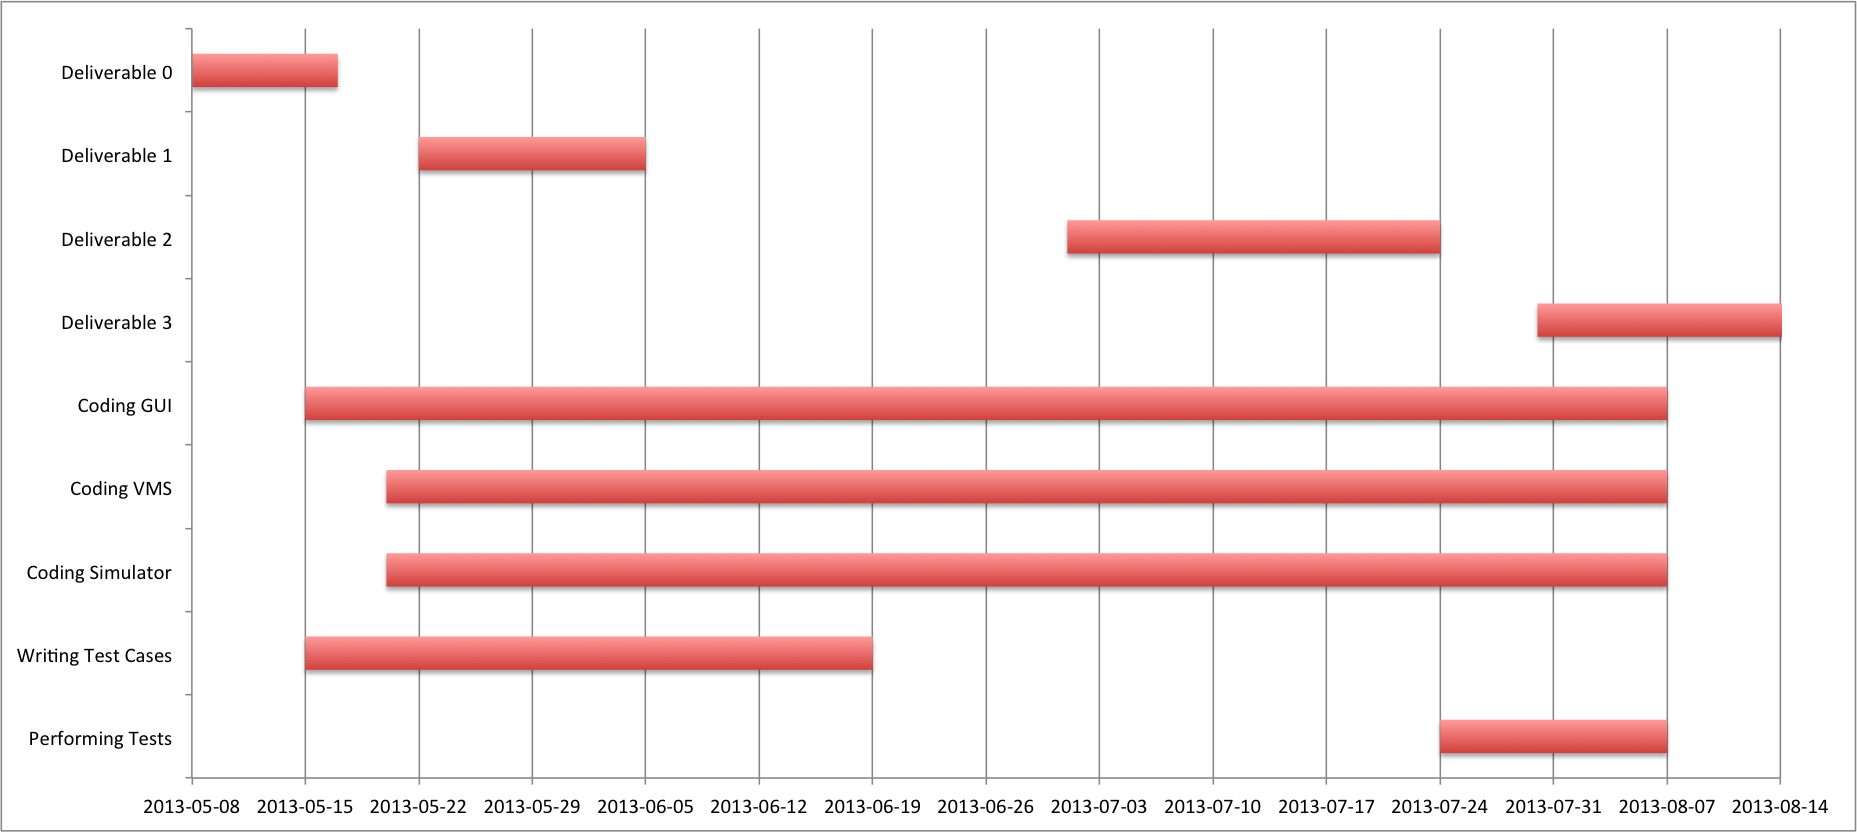
\includegraphics[scale=0.55]{charts/GanttChart.png}
\end{figure}

% Taken from last deliverable with only minor changes. Costs may have to be recalculated.
% \begin{description}

 %  \item[Simulator program:] \$150, cost to code and implement.
%   \item[VMS program:] \$150, cost to code and implement.
%   \item[Graphical User Interface:] \$100, cost to design, code, and implement.
%   \item[Unit test suite:] \$200, cost to write test cases and perform testing.
%   \item[Documentation:] \$250, includes all customer deliverables and internal documentation.
%   \item[Final integration:] \$90
%   \item[Buffer:] \$160
%   \item[Total Cost:] \$1100
% \end{description}
\clearpage
\begin{table}[ht]
\caption{Final Cost estimate table }
\centering

\begin{tabular}{|c |c |c| }
% centered columns (4 columns)
\hline \hline %inserts double horizontal lines
Components &  Estimate man Hours  &  Recorded man hours \\[0.1ex]
\hline
Deliverable 1 overview\\
\hline
Role assignment meeting	& 1&1\\
Proress work report	 & 2 & 2\\
Project description & 3&6\\
Goals and Constraints & 3& 6\\
Resource Evaluation & 3 & 6\\
Scoping and plan & 	3& 6\\
Diagram description Domain model, use cases &  1 & 2\\
Coding phase 1 & 8 & 8\\
Testing  & 4 & 5\\
Project design & 4 & 5\\
Total & 32 & 	47\\[1ex]
\hline
Deliverable 2 Overview\\
\hline		
Role assignment meeting &1 &1\\
Architectural design  Subsystem interfaces specs &3&3\\
Detailed design &3&2\\
Dynamic Design Scenarios	& 3&2\\
Program description Diagram  UMl digram & 6 & 7\\
Coding phase 2 & 6&6\\
Testing &4&2\\
Revision (cost estimation) & 1&1\\
Total &31&29\\
\hline
Deliverable 3 Overview \\
\hline		
Role Assignment meeting 	&1&	2\\
System delivery (user manual, admin manual)&5&5\\
Tested items 	&5&7\\
Test cases(units,requirements) &	10&10\\	
Code completion (fixing error and recoding)&	5&6\\
Finalizing the software to provide complete functional version & 5	&6\\
Final cost revision & 1 & 1\\
Total	&37&44\\
\hline
Project Total &100&130\\
\hline
\end{tabular}
\label{table:nonlin}
% is used to refer this table in the text
\end{table}

\paragraph{Basis} Costs have been calculated based on the amount of man hours spent working on project (at a normal approximate labor cost of \$15 an hour). There was no cost associated with tools, because all tools used were either freely available or were provided by the University.

\clearpage

\listoffigures
\clearpage

\end{document}
